\documentclass{article}
\newtheorem{theorem}{Theorem}[section]
\newtheorem{corollary}{Corollary}[theorem]
\newtheorem{lemma}[theorem]{Lemma}

\usepackage{listings}
\usepackage{color}
\usepackage{graphicx}
\usepackage{subcaption}
\usepackage{float}
\graphicspath{{./Figures/}}

\definecolor{dkgreen}{rgb}{0,0.6,0}
\definecolor{gray}{rgb}{0.5,0.5,0.5}
\definecolor{mauve}{rgb}{0.58,0,0.82}

\lstset{frame=tb,
  language=Python,
  aboveskip=3mm,
  belowskip=3mm,
  showstringspaces=false,
  columns=flexible,
  basicstyle={\small\ttfamily},
  numbers=none,
  numberstyle=\tiny\color{gray},
  keywordstyle=\color{blue},
  commentstyle=\color{dkgreen},
  stringstyle=\color{mauve},
  breaklines=true,
  breakatwhitespace=true,
  tabsize=3
}

\begin{document}
    \title{Linear Regression Model}
    \author{Youssef Allam}
    \maketitle

    \tableofcontents

    \newpage
    

    \section{Abstract}
        This project aims to implement a linear regression model from scratch without relying on any external libraries (with the exception of plotting purposes). The implementation will include desigining a \textit{Matrix} class which will perform all matrix operations needed for linear regression.
A sample of random input data as well as output data based on a pre-determined function with noise added to simulate real world data. The normal equation will be used to compute an approximate value for linear coeffecients which will then be used to approximate the output value for other inputs. Finally, The Mean Squared Error will be used to determine the accuracy of the model.
    
    \section{Theory of Linear Regression}
        \subsection{Goal of Linear Regression}
Regression is a statistical method that aims to determine the relationship between a set of inputs and their output.
Linear Regression is a form of regression that assumes the relationship is a linear relationship of the form:
\begin{equation}
    y=\sum_{k=1}^{n} \beta_k x_k
\end{equation}
n is the number of independent input variables each of which is denoted by $x_i$. 
$\beta$ is the $n\times1$ vector of coeffecients that we aim to determine. We will be given a matrix $X$ of inputs where for each row $i$ the entry $X_{ij}$ represents the value of $x_j$ in equation 1 for the $i$th input sample.
\\ \\$X_{ij}$ will be an $m \times{} n$ matrix containg the sample input data where m is the number of inputs and n is as defined above. The output vector $Y$ for the matrix of inputs will be given by \begin{equation}
    Y=X\beta+\epsilon
\end{equation} $Y$ will be an m dimensional vector containg the m respective outputs for m inputs and $\epsilon$ is the noise added to simulate real life inputs. \\ \\
One might think that the only issue with determining $Y$ is the noisy data but in reality another issue is that the matrix $X$ might be singular and overdetermines the solution. This is why we will use the least squares method to determine $\beta$.\\ \\
The goal of linear regression will be to determine an approximate numerical value for $\beta$ such that we can compute $\hat{Y}=X\beta$ for any given x where the hat denotes an approximate value.\\ \\
\subsection{Normal Equation Proof}
We will use equation 2 to solve for $\beta$. Our goal will be to minimize the square difference between $\hat{Y}$ and $Y$. We will define the error as:$E_i=(\hat{Y_i}-Y_i)^2$ for each $i$th input and we will aim to minimize $E$.
\begin{eqnarray}
    E=\sum_{i=1}^{m} E_i \nonumber \\
    E=\sum_{i=1}^{m} (\hat{Y_i}-Y_i)^2 \nonumber \\
    E=\sum_{i=1}^{m} (X_i\beta-Y_i)^2 \nonumber \\
    \frac{\partial{E}}{\partial{\beta}}=2(X_i\beta-Y_i)X_i=0 \nonumber \\
    X_i\beta X_i=Y_iX_i \nonumber \\
    X'X\beta=X'Y \nonumber \\
    \beta={(X'X)}^{-1}X'Y
\end{eqnarray}
To arrive at the final formula we had to use the inverse of $X'X$ for which we used the following lemma to be certain that $X'X$ is invertible.
\begin{lemma}
    For a given full column rank matrix $X$ the matrix $A=X'X$ is always invertible\\
    Refer to appendix for proof
\end{lemma}
We call the final equation The Normal Equation for linear Regression. \\
    
    \section{Matrices}
        \subsection{Matrix Representation}
We will use an array of arrays to represent a matrix. 
All of the processes will abstracted through a class \textit{Matrix} and we will add some
member functions such as \textit{print,peek,edit}, and\textit{square}
\begin{lstlisting}
class Matrix:
    def __init__(self,arroarr):
        check= True
        n=len(arroarr[0])
        for i in arroarr:
            if (len(i)!=n):
                check=False
        if(check):
            self.matrix = arroarr
            self.m = len(arroarr)
            self.n=len(arroarr[0])
        else:
            raise ValueError("Invalid Dimensions")

    def print(self):
        print('Rows: ',self.m,' Cols: ',self.n)
        for arr in self.matrix:
            for ind in arr:
                print(round(ind,5), end=" ")
            print("\n")

    def peek(self,row,col):
        if(row>self.m or col>self.n):
            raise ValueError("Out of Bounds")
        else:
            return self.matrix[row][col]

    def edit(self,row, col, val):
        if(row>self.m or col>self.n):
            raise ValueError("Out of Bounds")
        else:
            self.matrix[row][col]=val
    
    def square(self):
        return(self.m==self.n)

\end{lstlisting}
\subsection{Basic Matrix Operations}
Next we will overload the basic operators addition, subtraction, and multiplication with their respective definition in matrices.
\begin{lstlisting}
    def __add__(self, other):
        if(self.m==other.m and self.n==other.n):
            newmat = [[0] * self.n for i in range(self.m)]
            for i in range(0,self.m):
                for j in range(0,self.n):
                    newmat[i][j]=self.peek(i,j)+other.peek(i,j)
            result=Matrix(newmat)
            return result
        else:
            raise ValueError("Invalid Dimensions")

    def __sub__(self, other):
        if(self.m==other.m and self.n==other.n):
            newmat = [[0] * self.n for i in range(self.m)]
            for i in range(0,self.m):
                for j in range(0,self.n):
                    newmat[i][j]=self.peek(i,j)-other.peek(i,j)
            result=Matrix(newmat)
            return result
        else:
            raise ValueError("Invalid Dimensions")
    
    def __mul__(self, other):
        if(self.n!=other.m):
            raise ValueError("Invalid Dimensions")
            return
        result=[[0]*other.n for l in range(self.m)]
        for i in range(0,self.m):
            for j in range(0,other.n):
                result[i][j]=sum(self.matrix[i][k]*other.matrix[k][j] for k in range(0,other.m))
        R=Matrix(result)
        return R
\end{lstlisting}
\subsection{Row Operations}
Moving on we need to implement functions that perform basic row operations which are 
add (adds a multiple of a row to another row), 
scale(multiplies a row by a scaling factor),  
and exchange(exchange two rows together). 
 \begin{lstlisting}
    def row_scale(self,row,scale):
        if(row>self.m):
            raise ValueError("Out of Bounds")
        else:
            for i in range(0,self.n):
                self.matrix[row][i]=scale*self.matrix[row][i]

    def row_add(self,row1,row2,row2scale):
        if(row1>self.m or row2>self.m):
            raise ValueError("Out of Bounds")
        else:
            for i in range(0,self.n):
                self.matrix[row1][i]=self.matrix[row1][i]+row2scale*self.matrix[row2][i]

    def row_swap(self,row1,row2):
        if(row1==row2):
            return
        elif(row1>self.m or row2>self.m):
            raise ValueError("Out of Bounds")
        else:
            for i in range(0,self.n):
                temp=self.matrix[row1][i]
                self.matrix[row1][i]=self.matrix[row2][i]
                self.matrix[row2][i]=temp
 \end{lstlisting}
\subsection{Advanced Matrix Operations}
Finally we need to add functions to perform basic matrix operations such as Transpose, Row Reduction, and Inversion.\\
\\Transpose is a very simple procedure that returns the same matrix but after exchanging rows and columns
 \begin{lstlisting}
    def transpose(self):
        newmat=[[0]*self.m for i in range(self.n)]
        for i in range(0,self.m):
            for j in range(0,self.n):
                newmat[j][i]=self.peek(i,j)
        result=Matrix(newmat)
        return result
 \end{lstlisting}
Next we implement a function that returns the echelon form and row reduced echelon form of
the matrix. We will first use a function REF to reach echelon form then use that function in another function called RREF to row reduce it. 
We will also add a parameter (augment) which will be another matrix that the same row operations are performed on.
This addition will be very useful later on in calculating inverse matrices.
 \begin{lstlisting}
    def REF(self,augment=None):
        c_row=0
        c_col=0
        while(c_row<self.m and c_col<self.n):
            j=c_row
            while(self.matrix[j][c_col]==0):
                j=j+1
                if (j==self.m):
                    break
            if(j!=self.m):
                self.row_swap(j,c_row)
                if(augment):
                    augment.row_swap(j,c_row)
                for i in range(c_row+1,self.m):
                    coeff=-self.matrix[i][c_col]/self.matrix[c_row][c_col]
                    self.row_add(i,c_row,coeff)
                    if(augment):
                        augment.row_add(i,c_row,coeff)
                c_row=c_row+1
                c_col=c_col+1
            else:
                c_col=c_col+1



    def RREF(self,augment=None):
        self.REF(augment)
        c_row=self.m-1
        c_col=self.n-1
        while(c_row>=0 and c_col>=0):
            while(self.matrix[c_row][c_col]==0):
                c_col=c_col-1
            for i in range(c_row-1,-1,-1):
                coeff=-self.matrix[i][c_col]/self.matrix[c_row][c_col]
                self.row_add(i,c_row,coeff)
                if (augment):
                    augment.row_add(i, c_row, coeff)
            c_col = c_col - 1
            c_row = c_row - 1
        for i in range(self.m):
            coeff=1/self.matrix[i][i]
            self.row_scale(i,coeff)
            if(augment):
                augment.row_scale(i,coeff)
 \end{lstlisting}
 Finally we will implement an Inverse function that will be based on the Guass-Jordan method for computing inverse matrices where we will use the RREF and pass an identity matrix in the augment parameter.
 \begin{lstlisting}
    def inverse(self):
        temp=[[0]*self.m for i in range(self.m)]
        for k in range(self.m):
            for j in range(self.m):
                temp[k][j]=self.peek(k,j)
        T=Matrix(temp)
        if(T.square()==False):
            raise ValueError("Invalid Dimensions")
            return
        augment=[[0]*T.m for i in range (T.m)]
        for i in range (T.m):
            augment[i][i]=1
        A=Matrix(augment)
        T.RREF(A)
        return A
 \end{lstlisting}
    
    \section{Data Preparation}
        \subsection{Generating Input Data}
Next we need to prepare data to test our program. 
A function will be used to generate a matrix of sample inputs based on the desired sample size and the feature size. 
Feature size is the count of independent elements.
\begin{lstlisting}
    def generate_in(sample_size, feature_size):
        data=[[0]*feature_size for i in range(sample_size)]
        for i in range(sample_size):
            for j in range(feature_size):
                data[i][j]=np.random.randint(100)
        X=Matrix(data)
        return X
\end{lstlisting}
\subsection{Generating Output Data}
Another function will generate the output for the respective inputs genertaed above.
The function will be passed the sample input as well as a coeffecient matrix. 
Then noise will be added to the function to simulate real world conditions.

\begin{lstlisting}
    def generate_out(A,X):
        Y=X*A
        add_noise(Y,5)
        return Y

    def add_noise(A,max):
        for i in range(A.m):
            for j in range(A.n):
                A.matrix[i][j]=A.matrix[i][j]+np.random.rand()*max
\end{lstlisting}

    \section{Prediction and Plotting}
        \subsection{Single Variable Linear Regression}
We will first run our program on a single variable function of the form $y=5x_1$ through the following code.
\begin{lstlisting}
    ##Single Variable
    #GENERATE SAMPLE DATA
    X = generate_in(100, 1)
    Coeff = Matrix([[5]])
    Y = generate_out(Coeff, X)
    
    # SOLVE FOR BETA USING NORMAL EQUATION
    BETA = (X.transpose() * X).inverse() * X.transpose() * Y
    
    #Plot Sample Data and Predicted Values
    one_variable(Y,X,BETA)
    
\end{lstlisting}
This will generate a data sample of size 1000 and 1 feature with additional noise giving us data in figure 1(a). Next we will compute the line of best fit using BETA and plot the data and the line of best fit as shown in figure 1(b).   

\begin{figure}[h!]
    \centering
    \begin{subfigure}{0.5\textwidth}
        \centering
        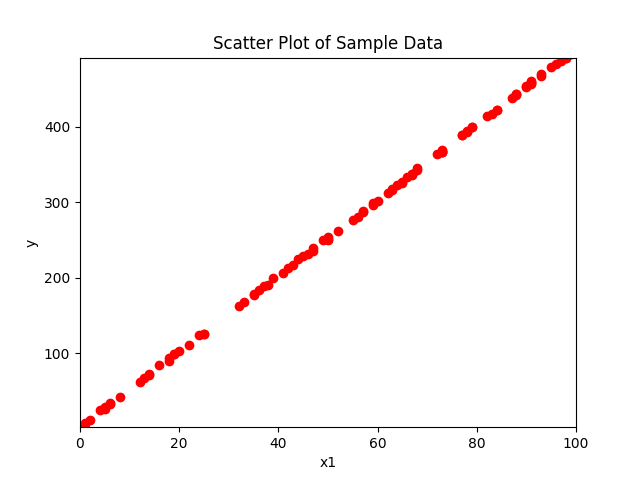
\includegraphics[scale=0.4]{One Variable Original.png}
        \caption{Original Data Set}
    \end{subfigure}%
    \begin{subfigure}{0.5\textwidth}
        \centering
        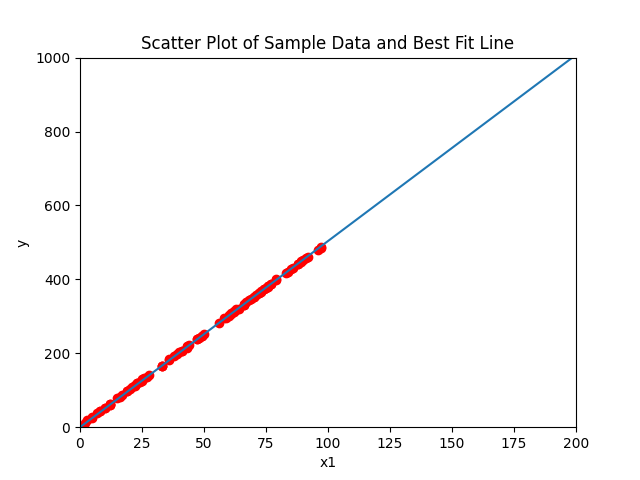
\includegraphics[scale=0.4]{One Variable Best Fit.png}
        \caption{Original Data Set and Line of Best Fit} 
    \end{subfigure}
    \caption{Single Variable Linear Regression}
\end{figure} 
\noindent The function \textit{one\_variable} which is responsible for plotting the data and the line of best fit is shown below.
\begin{lstlisting}
    def one_variable(Y,X,beta):
        x1 = [0] *(X.m)
        y=[0] *(Y.m)
        for i in range (X.m):
            x1[i]=X.matrix[i][0]
        for i in range (Y.m):
            y[i]=Y.matrix[i][0]
        ynew=[beta.matrix[0][0]*x1 for x1 in range(200)]
        plt.plot(x1,y,'ro')
        plt.plot([i for i in range(200)],ynew)
        plt.title('Scatter Plot of Sample Data and Best Fit Line')
        plt.xlabel('x1')
        plt.ylabel('y')
        plt.axis((0,200,0,1000))
        plt.show()
\end{lstlisting}


\subsection{Multi-Variable Linear Regression}
Next we will run our program for a multivariable function. Firstly we will generate data of sample size 1000 and 2 features.
We will use an equation of the form $y=5x_1+3x_2$ and generate sample outputs using the inputs and the coeffecients and use the normal equation to solve for BETA.
\begin{lstlisting}
    ##Multivariable
    #GENERATE SAMPLE DATA
    X=generate_in(1000,2)
    Coeff=Matrix([[5],[3]])
    Y=generate_out(Coeff,X)
    #SOLVE FOR BETA USING NORMAL EQUATION
    BETA=(X.transpose()*X).inverse()*X.transpose()*Y
    
    ##GRAPH CONTOUR PLOT
    mesh_grid(BETA)
    two_variable(X,Y)
\end{lstlisting}
We will use a contour plot to visualize the data and the approximation of the function. Figure 2(a) shows the original data set and figure 2(b) shows predicted values generated by linear regression.
\begin{figure}[H]
    \centering
    \begin{subfigure}{0.5\textwidth}
        \centering
        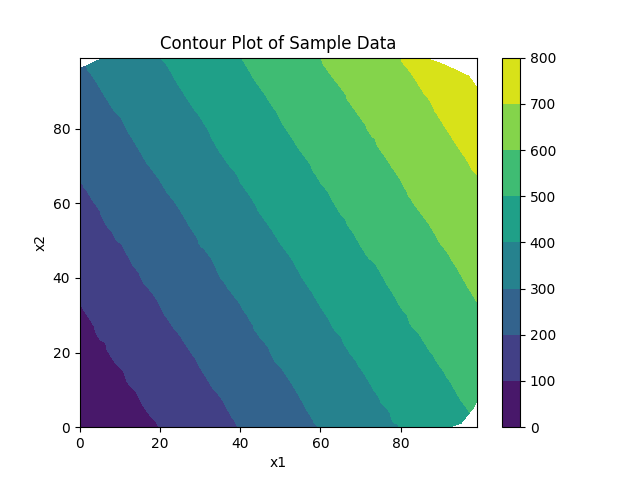
\includegraphics[scale=0.4]{Two Variable Original.png}
        \caption{Original Data Set}
    \end{subfigure}%
    \begin{subfigure}{0.5\textwidth}
        \centering
        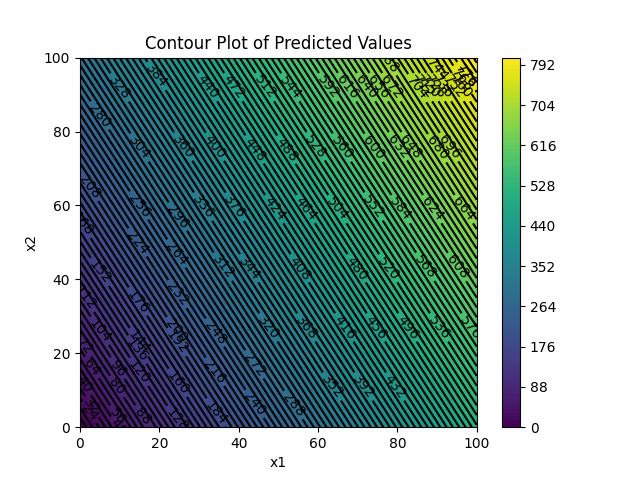
\includegraphics[scale=0.4]{Two Variable Predicted.png}
        \caption{Original Data Set and Predicted Values} 
    \end{subfigure}
    \caption{Multiple Variable Linear Regression}
\end{figure} 

\noindent The function \textit{two\_variable} will be used to plot the original sample data and the the function \textit{mesh\_grid} will be used to plot the contour plot of the predicted function both of which are shown below.
\begin{lstlisting}
    def mesh_grid(beta):
        x1=np.arange(0,101,1)
        x2=np.arange(0,101,1)
        X1,X2=np.meshgrid(x1,x2)
        Y=beta.matrix[0]*X1+beta.matrix[1]*X2
        ctr = plt.contour(X1, X2, Y, levels=100, colors='k')
        fil = plt.contourf(X1, X2, Y, levels=100)
        plt.clabel(ctr)
        plt.colorbar(fil)
        plt.show()

    def two_variable(X,Y):
        x1=[0]*X.m
        x2=[0]*X.m
        y = [0] * Y.m
        for i in range (X.m):
            x1[i]=X.matrix[i][0]
            x2[i]=X.matrix[i][1]
        for i in range (Y.m):
            y[i]=Y.matrix[i][0]
        plt.tricontourf(x1, x2, y)
        plt.colorbar()
        plt.show()
\end{lstlisting}

    \section{Evaluation}
        \subsection{MSE Evaluation}
Finally we need to find a way of evaluating the model. The most common way is through the mean square error.
The MSE is given by 
\begin{equation}
MSE=\frac{1}{N}\sum_{1}^{N}{(Y_i-\hat{Y_i})}^2
\end{equation}
Where N is the number of samples, $Y$ is the vector containing the original undistorted values and $Y_hat$ is the predicted values.
\begin{lstlisting}
#CALCULATE MSE
y_hat=[[0]*Y.n for i in range(Y.m)]
Y=X*Coeff
for i in range(X.m):
y_hat[i][0]=get_point(BETA,X.matrix[i][0],X.matrix[i][1])
Y_hat=Matrix(y_hat)
Diff=Y_hat-Y
MSE=sum((Diff.peek(i,0)*Diff.peek(i,0)) for i in range(Diff.m))/Diff.m
\end{lstlisting}
Though the MSE doesn't give us a way of knowing how accurate the model is in general it is a great way for comparing models. The MSE could be used to compare this model to other models or even to change parameters in this model and how these changes affect the model's error.
\subsection{Graphical Evaluation}
Anoher way we can evaluate our model in the above specific scenarios is by comparing the generated graphs to the original graphs since we already know the original function. This is a good way to evaluate the model as it gives us a visual representation of how well the model is doing. We show below the original and predicted graphs for the single variable and multi-variable functions.
\begin{figure}[h!]
        
    \centering
    \begin{subfigure}{0.5\textwidth}
        \centering
        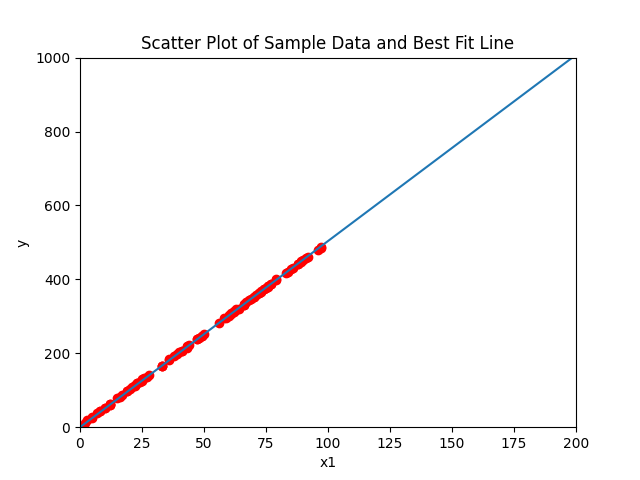
\includegraphics[scale=0.4]{One Variable Best Fit.png}
        \caption{Generated Best Fit Data}
    \end{subfigure}%
    \begin{subfigure}{0.5\textwidth}
        \centering
        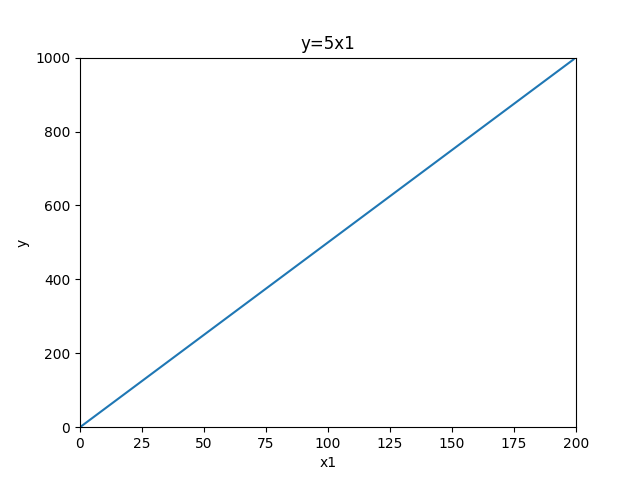
\includegraphics[scale=0.4]{One Variable Correct.png}
        \caption{Correct Best Fit Data}
    \end{subfigure}
    \caption{Comparison of Best Fit Data for Single Variable Linear Regression}
\end{figure}

\begin{figure}[!htb]
    \centering
    \begin{subfigure}{0.5\textwidth}
        \centering
        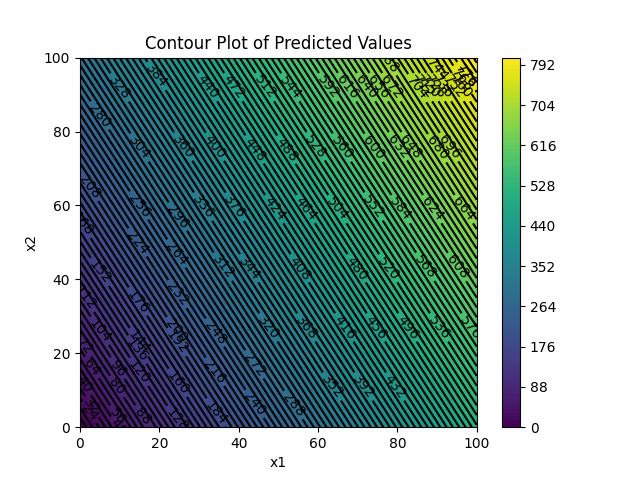
\includegraphics[scale=0.4]{Two Variable Predicted.png}
        \caption{Generated Best Fit Data}
    \end{subfigure}%
    \begin{subfigure}{0.5\textwidth}
        \centering
        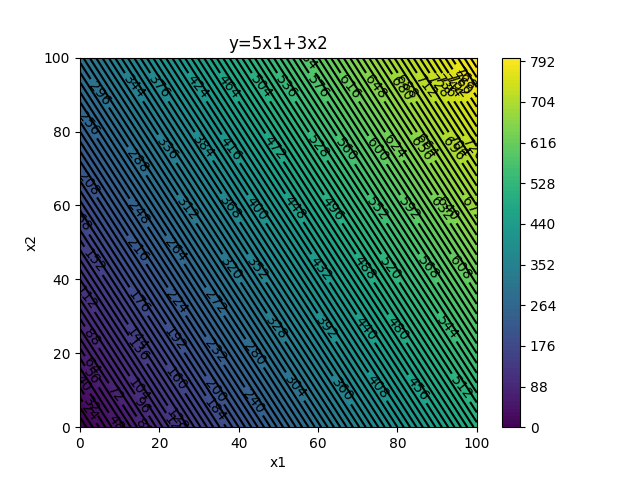
\includegraphics[scale=0.4]{Two Variable Corrected.png}
        \caption{Correct Best Fit Data}
    \end{subfigure}
    \caption{Comparison of Best Fit Data for Multivariable Linear Regression}
\end{figure}
    \section{Polynomial Regression}
        \subsection{Theory of Polynomial Regression}
The biggest drawback of Linear Regression is that it assumes linearity. To address this issue we will breifly discuss the concept of polynomial regression.
Polynomial Regression assumes that $y(x)=\sum_{i=0}^{n}a_{i}x^{i}$, where $n$ is the degree of the polynomial. This allows us to fit a curve to the data instead of a line$.$
In this case the data sample will simply be a vector of inputs $X$ and a vector of outputs $Y$. 
The inputs will be stored in a vandermonde matrix $V$ where $V_{ij}=X_{i}^{j}$. 
If the inputs $x_{i}$ are unique then the matrix $V$ will be invertible and the coefficients $a_{i}$ can be found by solving the system of equations $V\beta=Y$
otherwise, the system will be over determined and the least squares solution will be used. Furthermore, the data could be subject to noise which will not be an issue as the least squares solution will be used.
\\\\
We will use the same method we used before with the same Normal Equation to solve for $\beta$.
\begin{equation}
    \beta={(V'V)}^{-1}V'Y
\end{equation}
The only difference is that we will use the Vandermonde matrix $V$ instead of the input matrix $X$.
\subsection{implementation of Polynomial Regression from Linear Regression}
Since we already implemented linear regression we will just need to add some modifications to account for polynomial terms.
We will use a function to gernerate random input values and a function \textit{build\_poly} with parameters size and degree which will return the Vandermonde matrix of degree n for random input values of the given size.
\begin{lstlisting}
    def poly_samples(sample\_size):
        x=[0 for i in range (sample\_size)]
        for i in range(sample\_size):
            x[i]=np.random.randint(100)
        return x

    def build_poly(sample\_size,degree):
        samples=poly_samples(sample\_size)
        x=[[0]*(degree+1) for i in range(sample\_size)]
        for i in range(sample\_size):
            for j in range(degree+1):
                x[i][j]=pow(samples[i],j)
        X=Matrix(x)
        return X
\end{lstlisting}
Once we have generated sample input we will use an arbitrary function of $y=6x^2+3x+2$ to generate the output values and add noise to simulate real world data.
\begin{lstlisting}
    #Building Sample Data
    degree=2
    X=build_poly(1000,degree)
    coeff=[2,3,6]
    x = [0 for j in range(X.m)]
    for row in range(X.m):
        temp = 0
        x[row] = X.matrix[row][1]
    y=build_out(coeff,X)
    y=add_poly_noise(y,100)

    #Plotting Sample Data
    two_plot(x,y)
\end{lstlisting}
The functions \textit{build\_out} and \textit{add\_poly\_noise} are used to generate the output values and add noise respectively.
\begin{lstlisting}
    def build_out(Coeff,poly):
        y = [0 for j in range(poly.m)]
        x = [0 for j in range(poly.m)]
        for row in range(poly.m):
            temp = 0
            x[row] = poly.matrix[row][1]
            for i in range(poly.n):
                temp = temp + Coeff[i] * poly.matrix[row][i]
            y[row] = temp
        return y
    def add_poly_noise(y,max):
        for i in range(len(y)):
            y[i]=y[i]+np.random.rand()*max
        return y
\end{lstlisting}
Finally we will evaluate the coeffecients using the normal equation and plot the results of the curve fitting.
\begin{lstlisting}
    #Evaluating Coeffecients
    Y=Matrix([y])
    Y=Y.transpose()
    BETA = (X.transpose() * X).inverse() * X.transpose() * Y

    #Plotting Predicted Outcome
    x=[[0]*(degree+1) for i in range(200)]
    for i in range(200):
        for j in range(degree+1):
            x[i][j]=pow(i,j)
    X=Matrix(x)
    poly_plot(BETA.transpose().matrix[0],X)
\end{lstlisting}
The function \textit{poly\_plot} is used to plot the curve fitting.
\begin{lstlisting}
    def poly_plot(Coeff,X):
    y=[0 for j in range(X.m)]
    x=[0 for j in range(X.m)]
    for row in range(X.m):
        temp=0
        x[row]=X.matrix[row][1]
        for i in range(X.n):
            temp=temp+Coeff[i]*X.matrix[row][i]
        y[row]=temp
    plt.plot(x,y)
    plt.xlabel('x')
    plt.ylabel('y')
    plt.title('Curve Fit')
    plt.show()
\end{lstlisting}
The figure below shows the scatter plot of the sample data and the curve fitting.
\begin{figure}[h!]
    \centering
    \begin{subfigure}{0.5\textwidth}
        \centering
        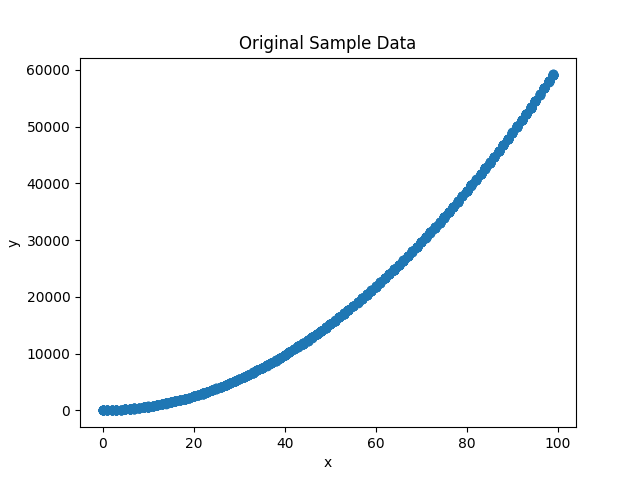
\includegraphics[width=\linewidth]{NonLinear Original.png}
        \caption{Sample Data}
    \end{subfigure}
    \begin{subfigure}{0.5\textwidth}
        \centering
        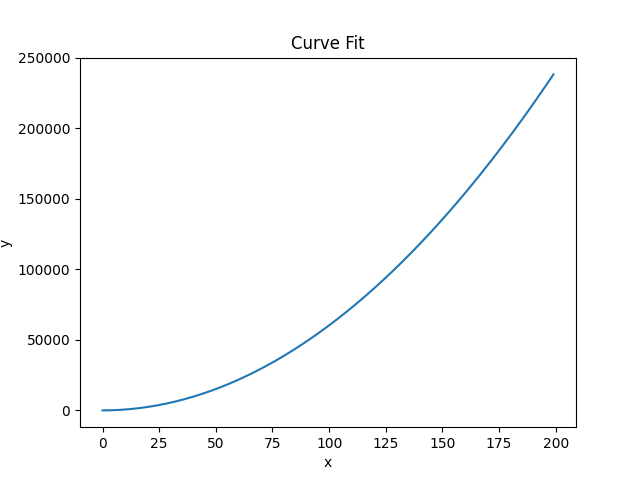
\includegraphics[width=\linewidth]{Non Linear Fit.png}
        \caption{Curve Fitting}
    \end{subfigure}
    \caption{Curve Fitting of Polynomial Regression}
\end{figure}
    
    \section{Conclusion}
        We now have the ability to use linear Regression to predict future values of any function given that we have enough sample data.
However linear regression does have some drawbacks the most major of which is that it assumes linearity when our original function could be a nonlinear function. This issue is addressed through Polynomial Regression as discussed in the previous section. However it still remains an issue to find the best function to fit this curve to and to what degree the polynomial should be.
Furthermore if you are dealing with real data there could be outliers which is why the data should be filtered to remove any anamoly before applying regression.
Despite all that linear regression is used in various industries and has various applications such as market analysis and sport analysis.

    \section{Appendix}
        \subsection{Proof of Lemma 2.1}
For a given matrix$m\times n$ matrix $A$ with full column rank, we will prove that the matrix $A^TA$ is invertible.\\
Full column rank would mean that the columns of $A$ are linearly independent and thus span the entire column space of $A$.\\
This would further imply that the matrix equation $Ax=0$ has only the trivial solution $x=0$.\\
We will now prove that $A^TA$ is invertible by proving that $A^TAx=0$ implies $x=0$.\\
\begin{eqnarray}
    A^TAx=0 \nonumber \\
    x^TA^TAx=0 \nonumber \\
    (Ax)^T(Ax)=0 \nonumber \\
    ||Ax||^2=0 \nonumber \\
    Ax=0 \nonumber \\
    x=0
\end{eqnarray}
Since we showed that $A^TAx=0$ implies $x=0$, we can conclude that $A^TA$ is invertible since it's columns must be linearly independent it is a square n matrix.\\


\end{document}